%!TEX root = main.tex

\section{Experimentation} % (fold)
\label{sec:experimentation}

\subsection{subsection name} % (fold)
\label{sub:subsection_name}
The first experiment that was attempted was measuring the binding energy of neutrons by observing the $\gamma$-ray emitted when the neutrons are captured by protons in the water surrounding a neutron source via reaction \ref{eq:neutronbinding},
\begin{align}
	\cf{^{1}_{1}p} + \cf{^{0}_{1}n} &\rightarrow \cf{^{1}_{2}d} + \gamma \label{eq:neutronbinding}
\end{align}

The exact energy would be found from the peak from this photon observed in the spectrum
% subsection subsection_name (end)

\subsection{Calibration} % (fold)
\label{sub:calibration}
Before any data can be read from the spectra taken from the detector, the data has to be calibrated. To do this, a set of known samples with well defined peaks is used to get a relation between the channel number of an observed peak and its energy. Once this is done, a relation can be found that relates the channel number to energy for use on later measurements.

The elements that were used included cobalt, barium, caesium, europium and americium. Each of these elements were available to measure, and each has recorded and accepted peaks that are at well defined positions. The data was taken from the National Nuclear Data Centre (NNDC). The table below shows the data that we collected from these sources. The channel number refers to the position in the spectrum that the peak was observed and the expected peak is the energy of the peak that the respective peak is estimated to correspond to.

\begin{table}[ht]
	\centering
	\begin{tabular}{r c|c|c}
		\multicolumn{2}{c|}{Element} & Channel Number & Expected Peak Energy (keV) \\
		\hline\hline
		Cobolt 		& $\ce{^{60}Co}$  & 369.4	& 1332.0 \\
					&				  & 324.9	& 1173.0	\\
		\hline
		Barium		& $\ce{^{133}Ba}$ & 102.9	& 356.0	\\
					&				  & 86.08	& 302.9		\\
		\hline
		Caesium		& $\ce{^{137}Cs}$ & 188.4	& 661.7 \\
		\hline
		Europium	& $\ce{^{152}Eu}$ & 99.84	& 344.3 \\
					&				  & 222.0	& 778.9		\\
					&				  & 274.9	& 964.1		\\
					&				  & 311.0	& 1121/1086	\\
					&				  & 394.1	& 1408.0	
	\end{tabular}
	\caption{This table shows some data\label{tab:myfirsttable}}
\end{table}
From these, the graph in figure \ref{fig:naicalib} can be drawn which shows the relation that can be used as a calibration between energy and channel number. The exact value of this relation, intercept and gradient, are subject to change since the calibration is retaken at the start of each session to account for changes in the experimental set-up and the radioactivity of the source which will decrease with time.

\begin{figure}[ht]
	\centering
	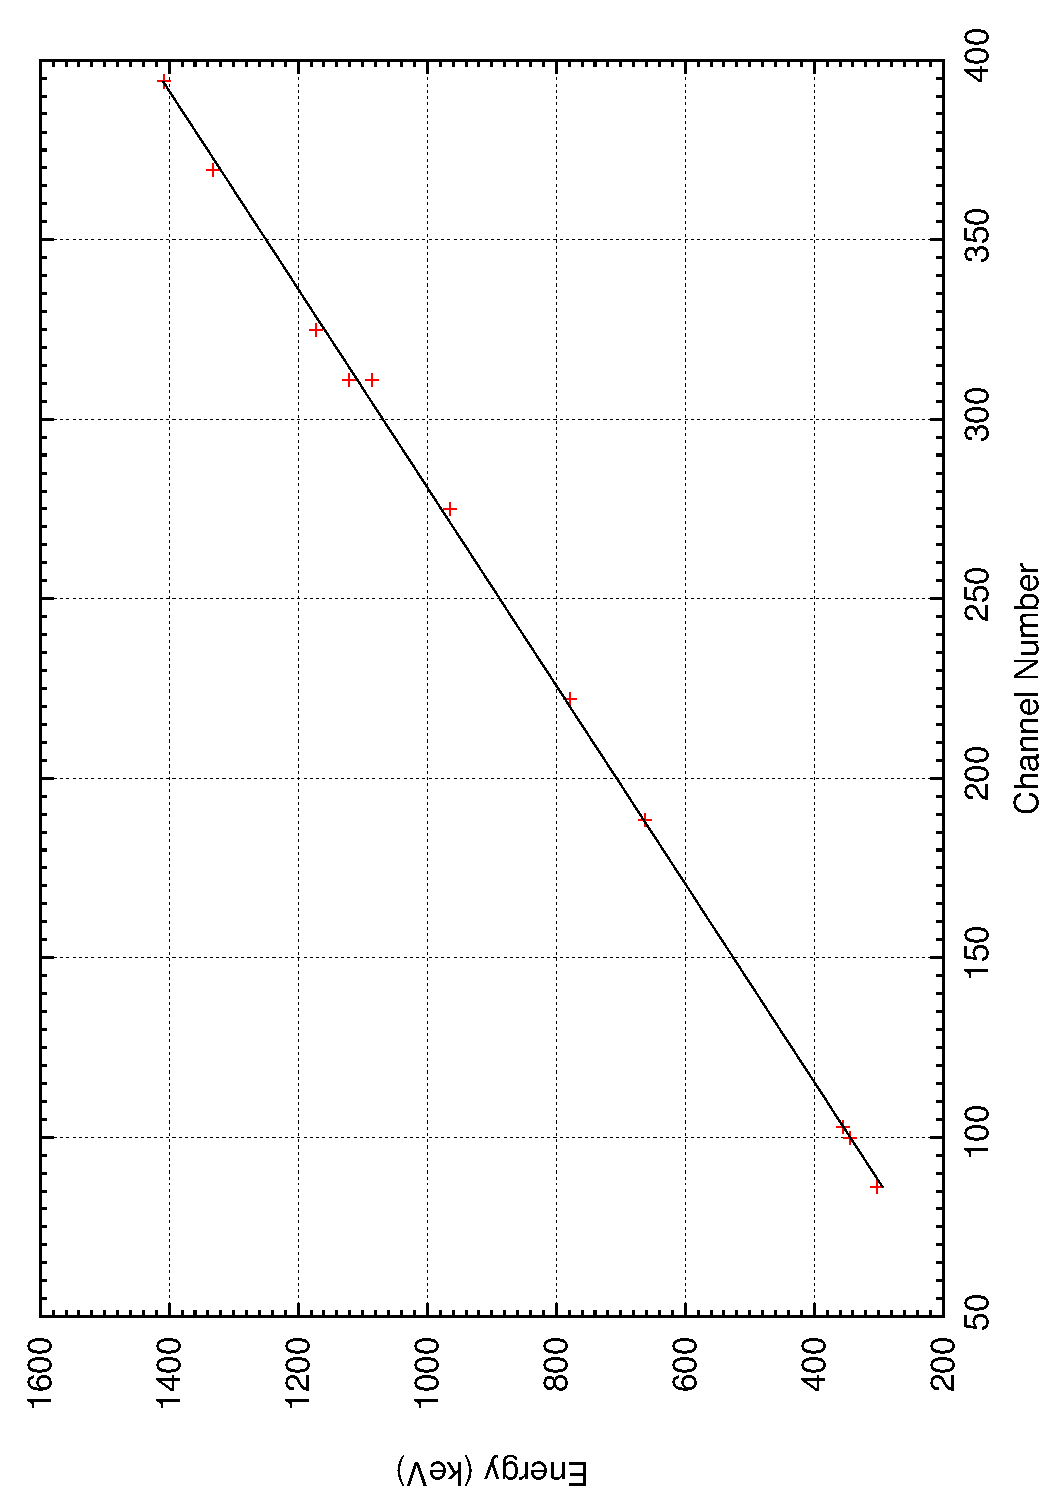
\includegraphics[angle=270,width=0.8\textwidth]{calibration1NaI.pdf}
	\caption{The $\text{BF}_4$ detector uses a high charge to create a flow of ions to measure the incoming neutron. It cannot measure the energy, but simply gives a count for the number of neutrons incident in the detector.\label{fig:naicalib}}
\end{figure}
An example of the spectra from the sources is shown in figure \ref{fig:cobaltcalib}. This shows the spectrum of $\ce{^{60}Co}$ which has been fitted with the Gaussian peaks to find the position and FWHM using the ``root'' package.

\begin{figure}[ht]
	\centering
	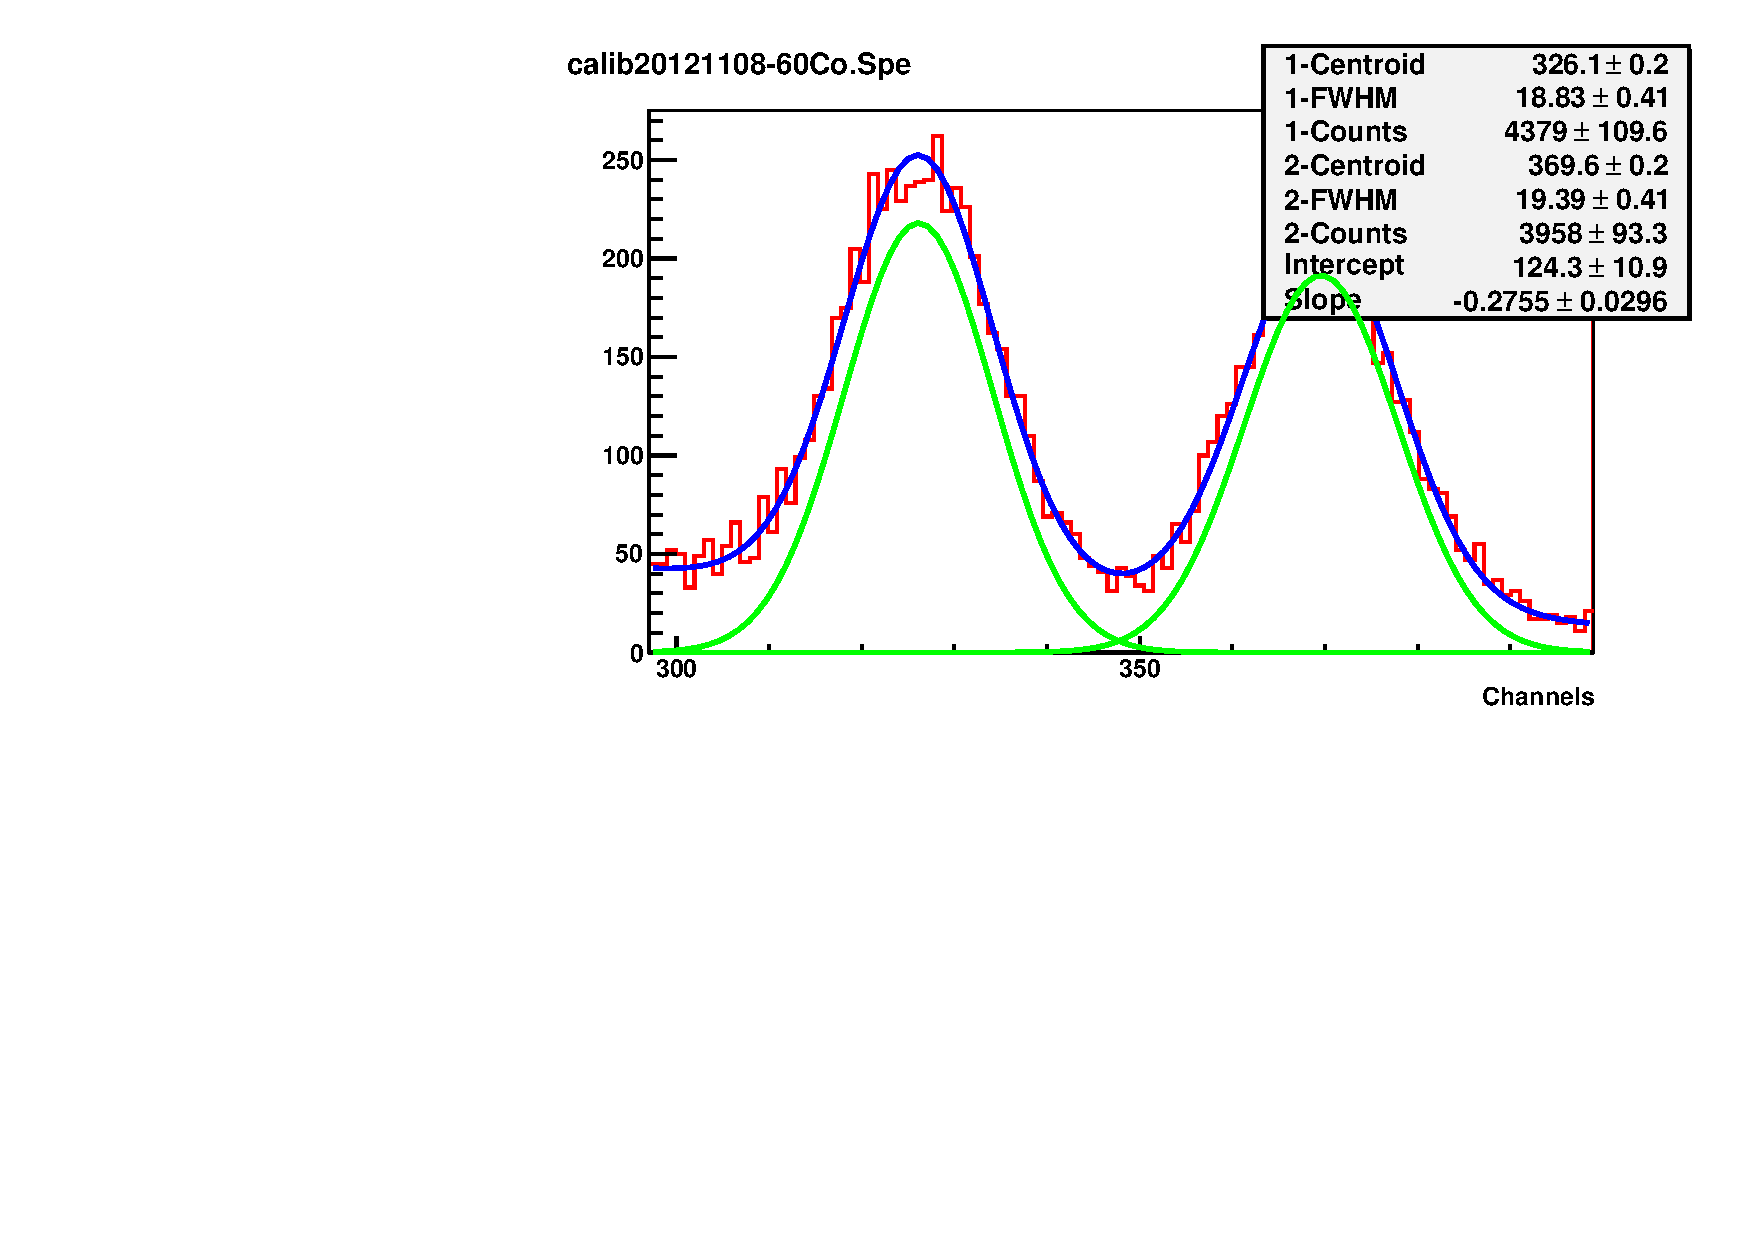
\includegraphics[angle=270,width=0.8\textwidth]{calib20121113-60Co.pdf}
	\caption{The $\text{BF}_4$ detector uses a high charge to create a flow of ions to measure the incoming neutron. It cannot measure the energy, but simply gives a count for the number of neutrons incident in the detector.\label{fig:naicalib}}
\end{figure}
% subsection calibration (end)
% section experimentation (end)
